\section{Introduction}


\begin{frame}{Introduction}\framesubtitle{Édition collaborative}

  L'édition collaborative concerne toutes les activités effectuées en
  \textbf{groupe} dans le but de produire un \textbf{document}. L'effort
  collectif permet de bénéficier de multiples points de vues différents.

  \begin{itemize}
  \item[$\rightarrow$] Les documents sont de \textbf{meilleure qualité}.
  \end{itemize}
  
  \vspace{1cm}

  \begin{minipage}{0.6\textwidth}
    \textit{La version anglaise de Wikipédia compte \textbf{5 millions}
      d'articles, \textbf{40 millions} de pages et \textbf{112 mille}
      utilisateurs actifs.\vspace{0.15cm}\\Les articles possèdent une
      \textbf{fiabilité} \textbf{comparable} à celle de l'Encyclopædia
      Britannica.}
  \end{minipage}\footfullcite{giles2005internet}
  \hfill
  \begin{minipage}{0.3\textwidth}
    \begin{figure}
      \begin{center}
        
\includegraphics[width=0.7\textwidth]{img/wikipedia.png}
      \end{center}
    \end{figure}
  \end{minipage}

\end{frame}


\begin{frame}{Introduction}{Éditeur collaboratif}
%  \begin{minipage}{0.53\textwidth}
%     Un éditeur collaboratif permet
%     \begin{itemize}
%     \item à \textbf{plusieurs personnes}
%     \item de \textbf{lire} et \textbf{modifier} un document.
%       % \begin{itemize}
%       % \item \textbf{ajout} de caractères
%       % \item \textbf{suppression} de caractères
%       % \end{itemize}
%     \end{itemize}
    
%     Grâce au Web,
%     \begin{itemize}
%     \item n'importe quel outil accédant à l'internet (\textit{e.g. ordinateur,
%         smartphone, tablette}) permet de créer et d'éditer un document aisément.
%     \item Un simple lien permet de le partager facilement avec des amis ou des
%       collègues.
%     \end{itemize}    
% %  \end{minipage}
% %  \begin{minipage}{0.45\textwidth}
%     \begin{figure}    
%       \begin{center}
%         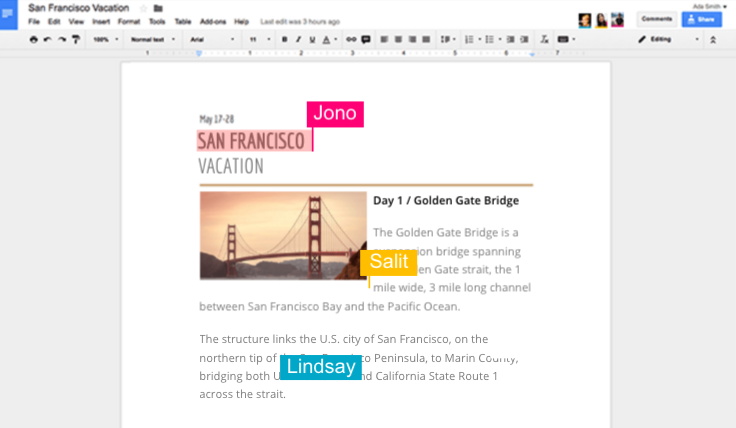
\includegraphics[width=0.65\textwidth]{img/googledocs.png}
% %        \caption{Capture d'écran d'un document Google Docs rédigé par 3 personnes
% %          en simultané. \REF}
%       \end{center}
%     \end{figure}
%  \end{minipage}
  
  \begin{textblock*}{\textwidth}(-1cm,-2.5cm) 
    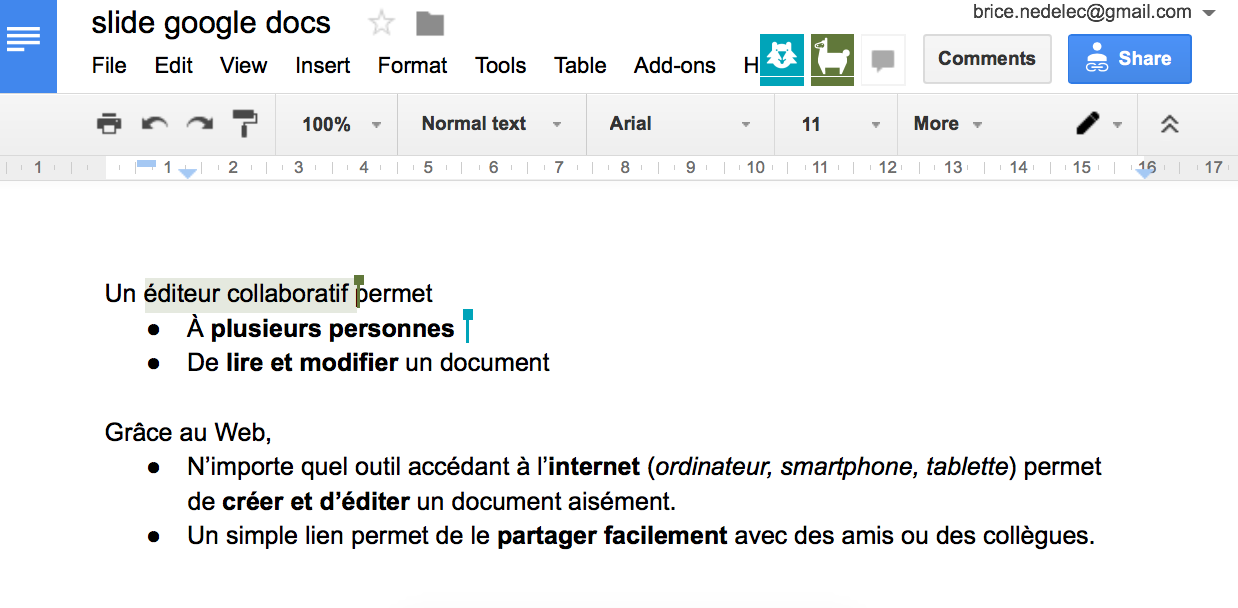
\includegraphics[width=1.19\textwidth]{img/googledocs3.png}
    % \footfullcite{johansen1988groupware}
%    \vspace{0.25cm}
  \end{textblock*}

  \begin{textblock*}{\textwidth}(0cm,4cm)
    \large
    \begin{itemize}
    \item[$\Rightarrow$] L'édition \textbf{temps réel} et le \textbf{Web}
      contribuent grandement à la popularité de tels éditeurs.
    \end{itemize}    
  \end{textblock*}
\end{frame}


\begin{frame}{Introduction}{Le contexte Web incite à la centralisation}
  
%  \hspace{-1cm}
  \begin{minipage}{0.69\textwidth}
    Problèmes de \textbf{confidentialité}, \textbf{censure},
    \textbf{intelligence économique}, \textbf{legislation}, etc. \vspace{0.15cm}\\
    \small\textit{En 2013, les révélations sur PRISM montre que la NSA possède des
      accès aux données hébergées par Google, Facebook, YouTube, Microsoft,
      Yahoo!, Skype, AOL et Apple.}
  \end{minipage}
  \hfill
  \begin{minipage}{0.3\textwidth}
    \hfill
    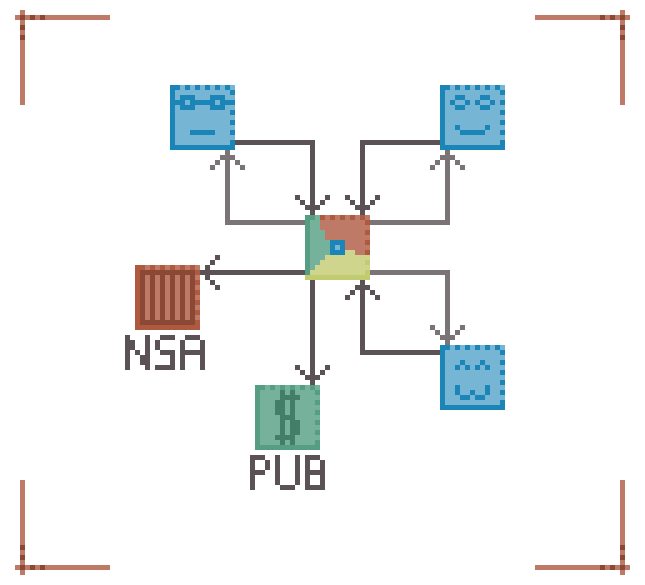
\includegraphics[width=0.97\textwidth]{img/centralizedethicproblems.png}
  \end{minipage}

  \begin{minipage}{0.69\textwidth}
    Problèmes de passage à l'échelle, notamment en \textbf{nombre de
      collaborateurs}. \vspace{0.15cm}\\
    \small\textit{En 2013, Coursera rassembla 41000 étudiants sur un seul cours.  Les
      limitations de l'outil collaboratif utilisé conduisirent au \og
      désastre\fg.}% \footfullcite{strauss2013how}.}
  \end{minipage}
  \hfill
  \begin{minipage}{0.3\textwidth}
    \hfill
    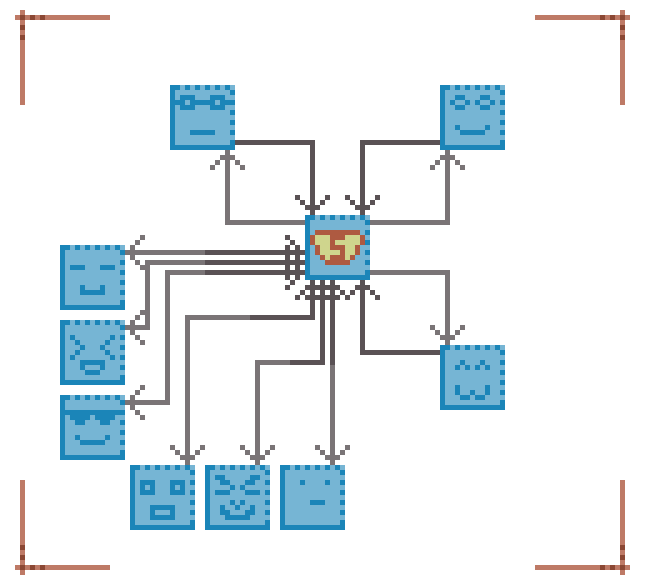
\includegraphics[width=0.97\textwidth]{img/centralizedcpuproblems.png}
  \end{minipage}

  \begin{minipage}{0.69\textwidth}
    Problèmes de \textbf{robustesse face aux défaillances}.
  \end{minipage}
  \hfill
  \begin{minipage}{0.3\textwidth}
    \hfill
    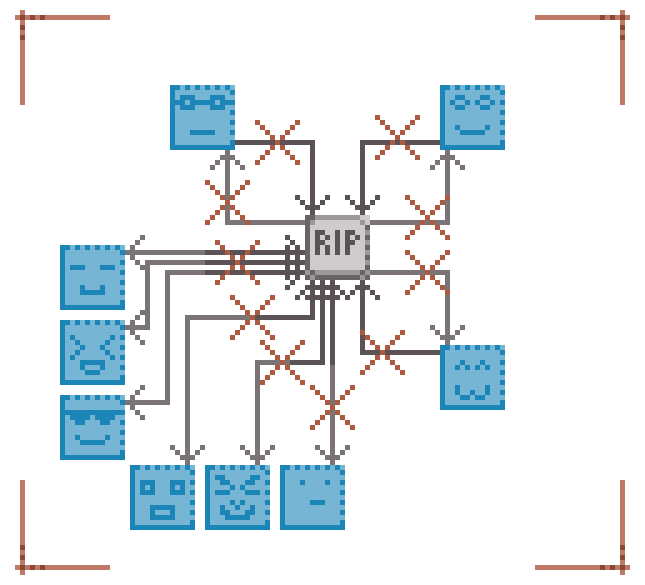
\includegraphics[width=0.97\textwidth]{img/centralizedscalabilityproblems.png}
  \end{minipage}

\end{frame}


\begin{frame}{Introduction}{Ce que l'on veut : un éditeur collaboratif \ldots}
  
%  \begin{textblock*}
  \begin{minipage}{0.45\textwidth}
    \hfill \YES{\cmark} \textbf{Temps réel}
  \end{minipage}
  \begin{minipage}{0.45\textwidth}
    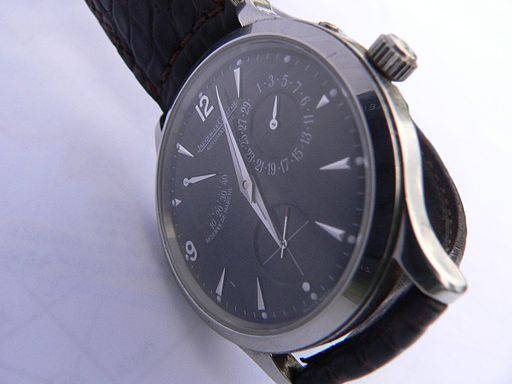
\includegraphics[width=0.75\textwidth]{img/watch.jpg}
  \end{minipage}
  % \end{textblock*}
    
  \vspace{-0.75cm}

  \begin{minipage}{0.45\textwidth}
    \hfill  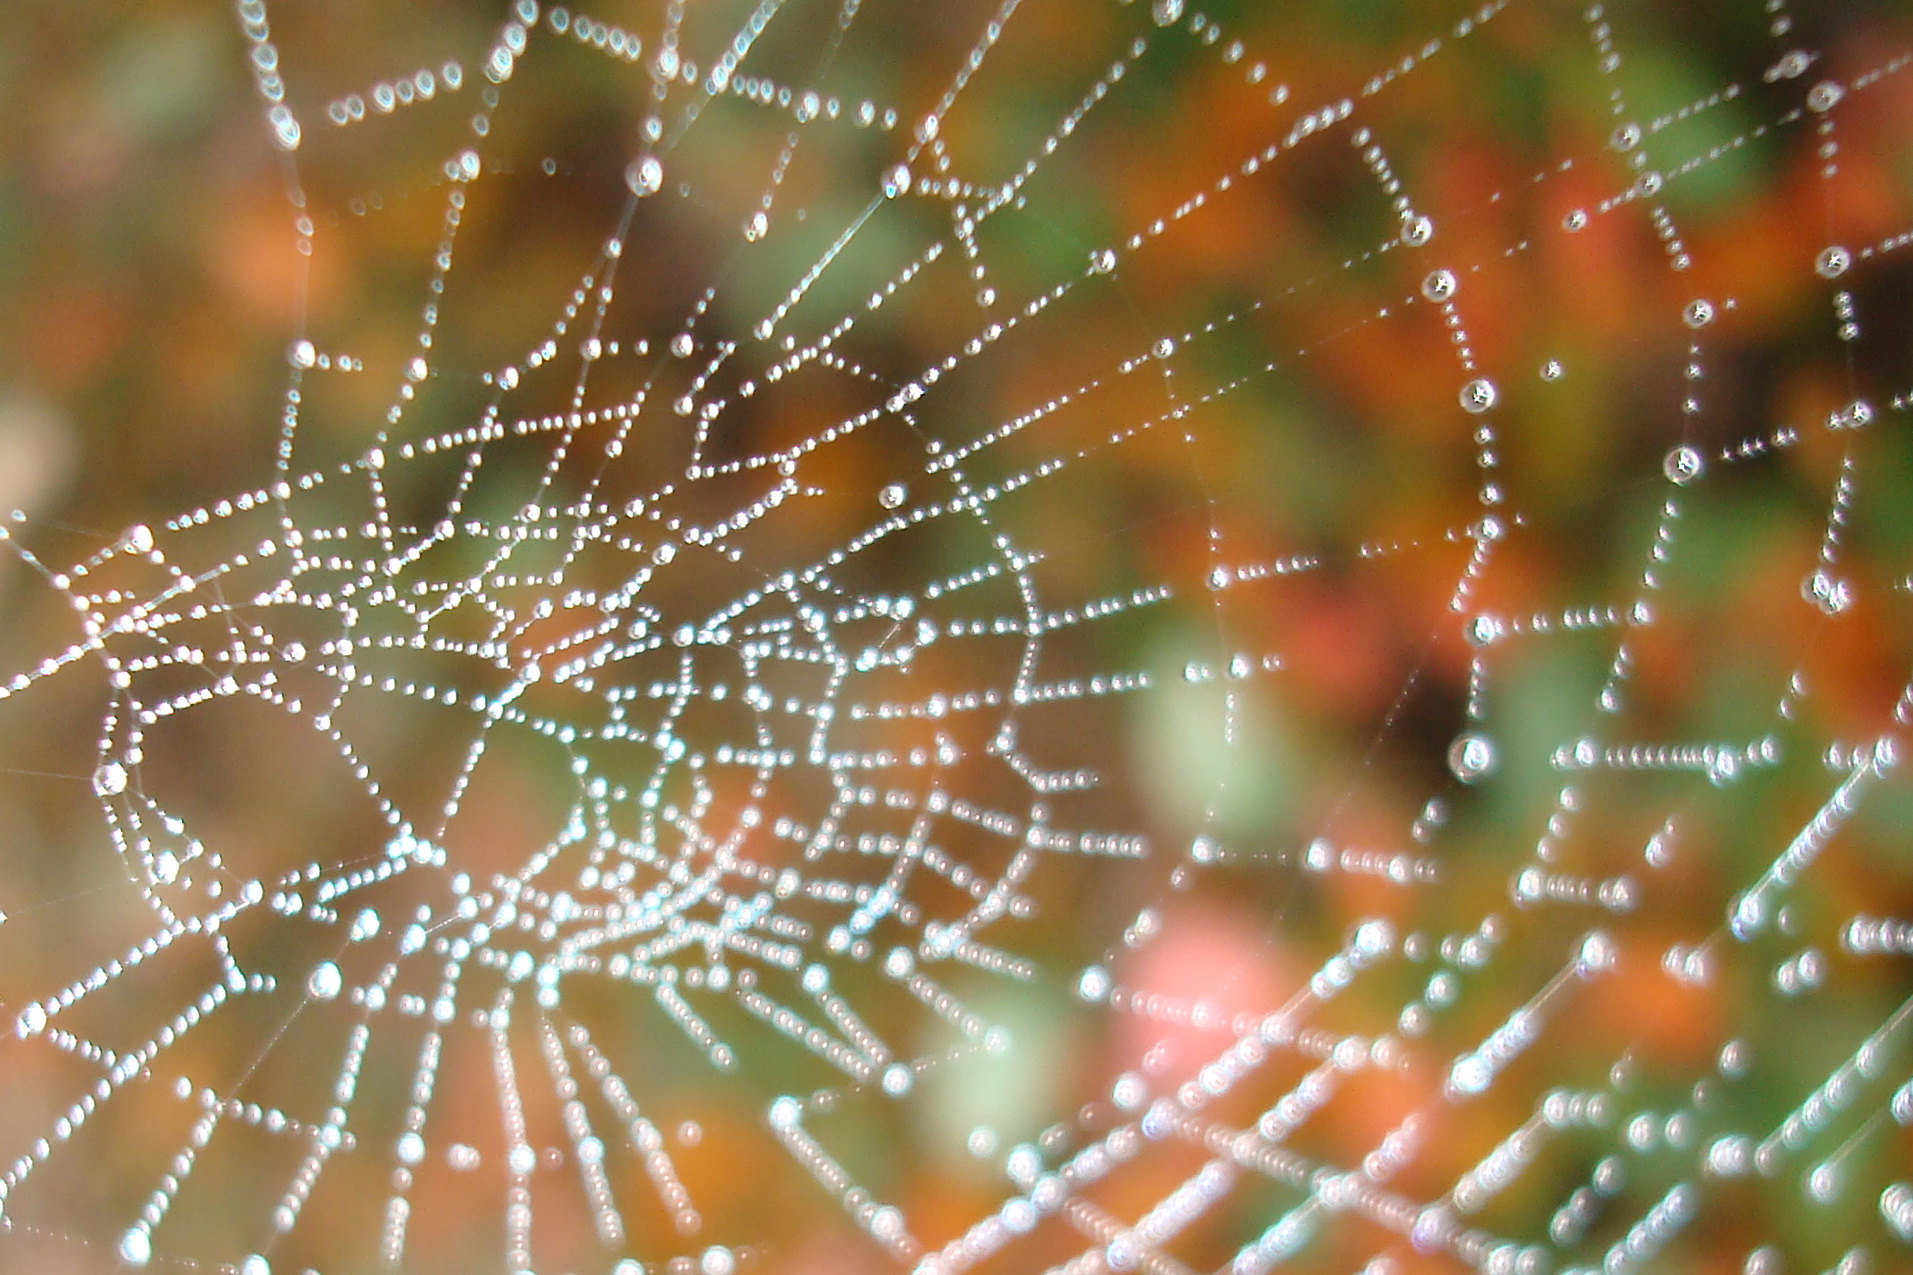
\includegraphics[width=0.8\textwidth]{img/toile.jpg}
  \end{minipage}  
  \begin{minipage}{0.45\textwidth}
    \textbf{Web} \YES{\cmark}
  \end{minipage}
  
  \vspace{-0.75cm}
  
  \begin{minipage}{0.45\textwidth}
    \hfill \NO{\xmark}\textbf{Sans fournisseur de services}
  \end{minipage}
  \begin{minipage}{0.45\textwidth}
    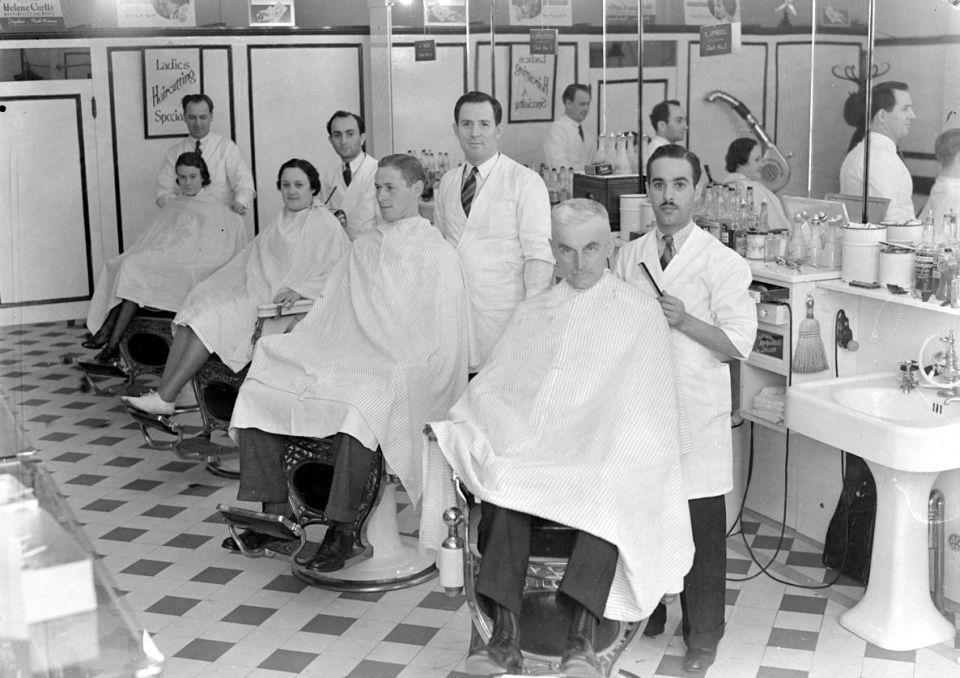
\includegraphics[width=0.8\textwidth]{img/service.jpg}
  \end{minipage}

  \vspace{-0.75cm}

  \begin{minipage}{0.45\textwidth}
    \hfill 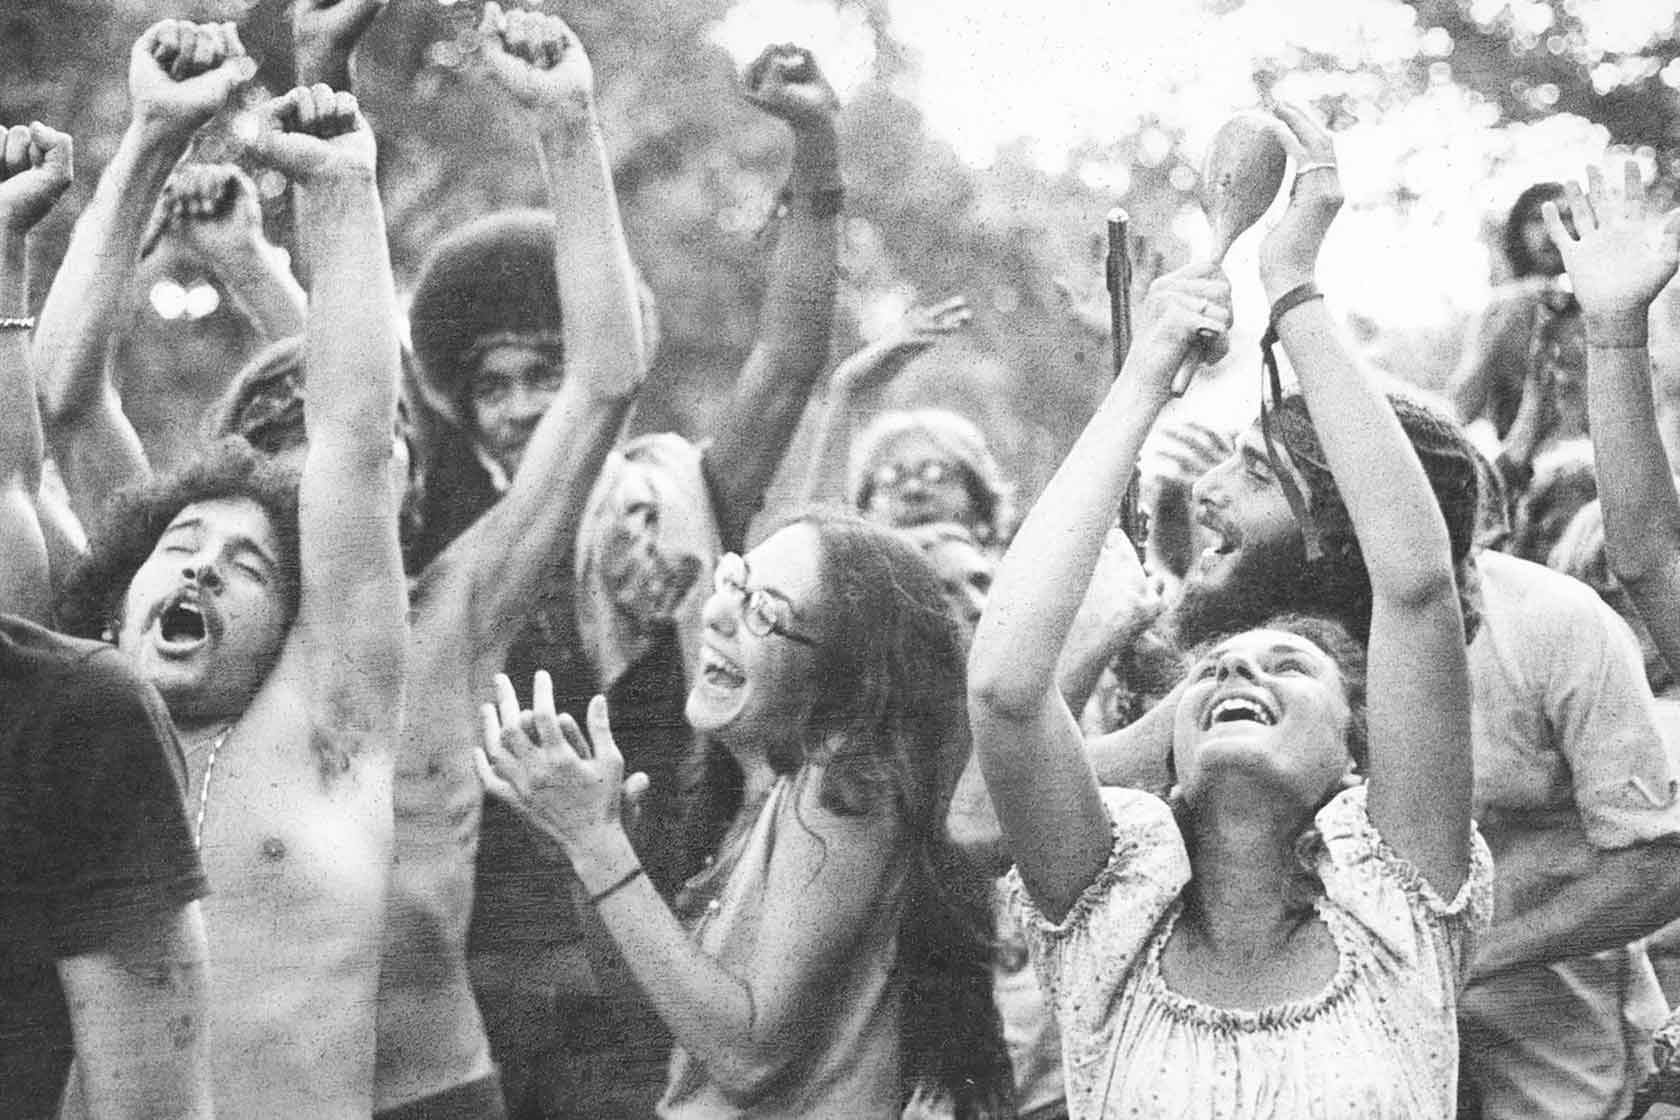
\includegraphics[width=0.8\textwidth]{img/crowd.jpg}
  \end{minipage}
  \begin{minipage}{0.45\textwidth}
    \textbf{Des milliers d'utilisateurs éditant simultanément} \NO{\xmark}
  \end{minipage}

\end{frame}


\begin{frame}{Introduction}{Un éditeur décentralisé dans les navigateurs}
  

  \begin{minipage}{0.69\textwidth}
    \CRATE est un éditeur collaboratif 
    \begin{itemize}
    \item temps réel \YES{\cmark}
    \item fonctionnant dans les navigateurs Web \YES{\cmark}
    \item sans fournisseur de services \YES{\cmark}
    \item pouvant atteindre de large dimensions \YES{\cmark}
    \end{itemize}
  \end{minipage}
  \begin{minipage}{0.3\textwidth}
    
\includegraphics[width=\textwidth,interpolate=false]{img/crateicon.png}
  \end{minipage}
    
%  \vspace{1.0cm}
  
  \begin{textblock*}{1.18\textwidth}(-1cm,1cm)
    \animategraphics[loop,autoplay,width=1\textwidth]{10}{img/animations/tmp-}{0}{69}
  \end{textblock*}
  
  \vspace{1cm}

\end{frame}


\begin{frame}{Introduction}\framesubtitle{Éditeur collaboratif décentralisé}
  
  \begin{center}
    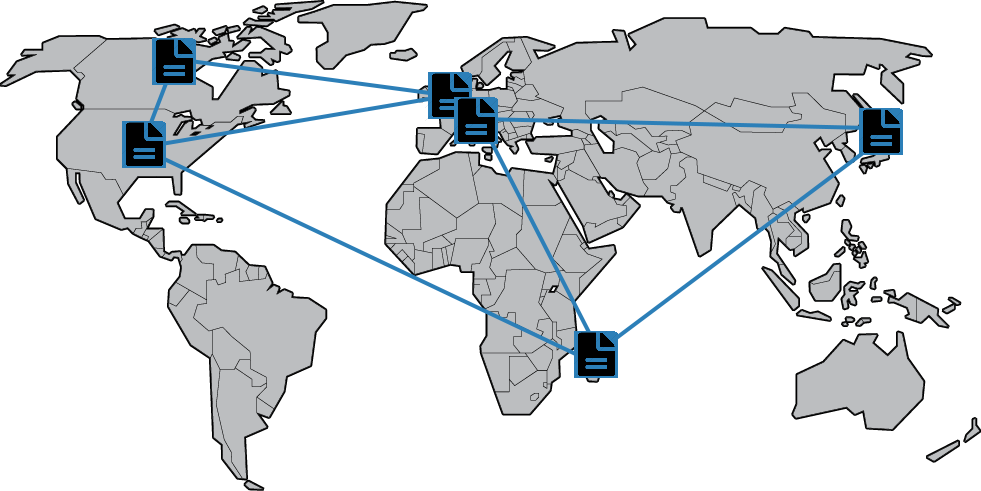
\includegraphics[width=0.8\textwidth]{img/world.png}
  \end{center}

  \vspace{0.25cm}

  \begin{itemize}
  \item [$\rightarrow$] Un éditeur collaboratif doit fonctionner sur les outils
    informatiques les plus modestes (CPU, mémoire, \textbf{largeur de bande}).
    \begin{itemize}
    \item [$\rightarrow$] (taille des messages $\times$ nombre de messages)
    \end{itemize}
  \end{itemize}

  \vspace{0.25cm}
  
  \begin{enumerate}
  \item Moyen de représenter efficacement un \textbf{document} de manière
    \textbf{cohérente}; %\small{$\rightarrow$ taille des messages}
  \item Moyen de \textbf{communiquer} efficacement les modifications sur le
    document. %\small{$\rightarrow$ nombre de messages}
  \end{enumerate}


  % \begin{itemize}
  % \item Répartition géographique des collaborateurs;
  % \item Édition en temps réel.
  % \end{itemize}
\end{frame}


%%% Local Variables:
%%% mode: latex
%%% TeX-master: "../slides"
%%% End:
